\documentclass[border=10pt]{standalone}
\usepackage[svgnames]{xcolor}
\usepackage{amsmath}
\usepackage{pgfplots}
\pgfplotsset{compat=newest}
\usepackage[sfdefault]{FiraSans}
\usepackage{FiraMono}
\renewcommand*\familydefault{\sfdefault}
\begin{document}
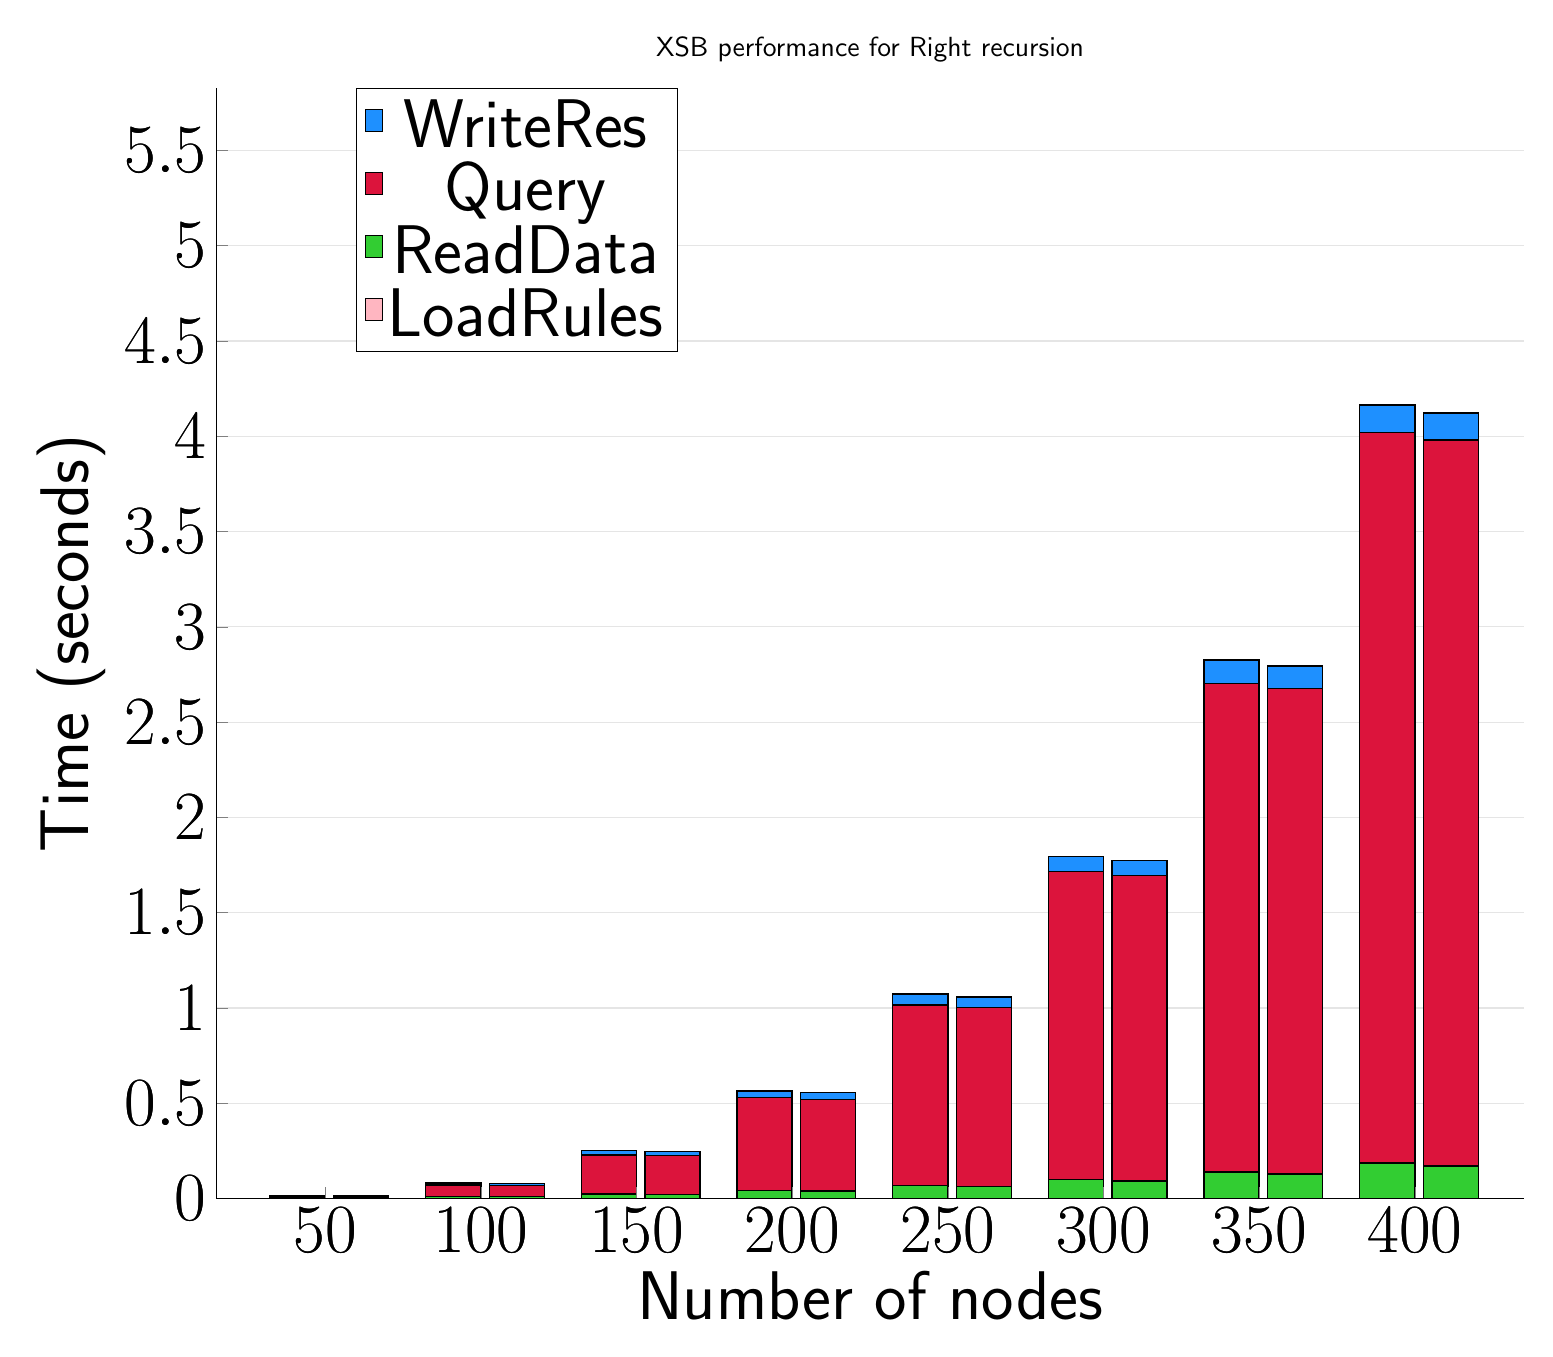
\begin{tikzpicture}
\begin{axis}[
   ybar stacked,
   title={XSB performance for Right recursion},
   bar shift=-10pt,
   width=1.5\textwidth,
   bar width=0.7cm,
   ymajorgrids, tick align=inside,
   major grid style={draw=gray!20},
   xtick=data,
   ymin=0, ymax=5.828503680229188,
   axis x line*=bottom,
   axis y line*=left,
   enlarge x limits=0.1,
   legend style={
       at={(0.23, 1)},
       anchor=north,
       legend columns=1,
       font=\Huge,
   },
   ylabel={Time (seconds)},
   xlabel={Number of nodes},
   label style={font=\Huge},
   tick label style={font=\Huge},
]
\addlegendimage{fill=DodgerBlue, draw=black, line width=0.2pt}
\addlegendentry{WriteRes}
\addlegendimage{fill=Crimson, draw=black, line width=0.2pt}
\addlegendentry{Query}
\addlegendimage{fill=LimeGreen, draw=black, line width=0.2pt}
\addlegendentry{ReadData}
\addlegendimage{fill=LightPink, draw=black, line width=0.2pt}
\addlegendentry{LoadRules}
\addplot +[fill=LightPink, draw=black, line width=0.5pt] coordinates {
    (50, 0.0009774208068847638)
    (100, 0.0010820388793945318)
    (150, 0.001067757606506349)
    (200, 0.0010587930679321288)
    (250, 0.0010821342468261708)
    (300, 0.001097989082336427)
    (350, 0.0011214017868041988)
    (400, 0.001176071166992188)
};
\addplot +[fill=LimeGreen, draw=black, line width=0.5pt] coordinates {
    (50, 0.002818989753723146)
    (100, 0.009945702552795414)
    (150, 0.02262160778045655)
    (200, 0.042183494567871085)
    (250, 0.06786463260650635)
    (300, 0.09917488098144531)
    (350, 0.13867335319519053)
    (400, 0.18474340438842768)
};
\addplot +[fill=Crimson, draw=black, line width=0.5pt] coordinates {
    (50, 0.007891488075256348)
    (100, 0.06044020652770996)
    (150, 0.204933190345764)
    (200, 0.48612258434295647)
    (250, 0.9469062089920046)
    (300, 1.61514699459076)
    (350, 2.563583755493163)
    (400, 3.833530688285825)
};
\addplot +[fill=DodgerBlue, draw=black, line width=0.5pt] coordinates {
    (50, 0.0025632143020630034)
    (100, 0.00944700241088868)
    (150, 0.024338817596435802)
    (200, 0.034828734397888306)
    (250, 0.05700950622558663)
    (300, 0.08068509101867602)
    (350, 0.12346463203430295)
    (400, 0.1446080923080471)
};
\end{axis}
\begin{axis}[
   ybar stacked,
   bar shift=13pt,
   width=1.5\textwidth,
   bar width=0.7cm,
   ymajorgrids, tick align=inside,
   major grid style={draw=none},
   xtick=data,
   ymin=0, ymax=5.828503680229188,
   axis x line*=none,
   axis y line*=none,
   enlarge x limits=0.1,
   label style={font=\Huge},
   tick label style={font=\Huge},
]
\addplot +[fill=LightPink, draw=black, line width=0.5pt] coordinates {
    (50, 0.0005436999999999999)
    (100, 0.0006297)
    (150, 0.0006088999999999999)
    (200, 0.0006082000000000001)
    (250, 0.0006123999999999998)
    (300, 0.0006215000000000003)
    (350, 0.0006266999999999999)
    (400, 0.0006372000000000003)
};
\addplot +[fill=LimeGreen, draw=black, line width=0.5pt] coordinates {
    (50, 0.0023761999999999998)
    (100, 0.0088507)
    (150, 0.0206731)
    (200, 0.0383251)
    (250, 0.061571799999999996)
    (300, 0.0910103)
    (350, 0.12799129999999997)
    (400, 0.1706672)
};
\addplot +[fill=Crimson, draw=black, line width=0.5pt] coordinates {
    (50, 0.0077931)
    (100, 0.059859300000000004)
    (150, 0.20364539999999995)
    (200, 0.48165009999999997)
    (250, 0.9390012999999999)
    (300, 1.6043246)
    (350, 2.5467262000000006)
    (400, 3.8088134000000005)
};
\addplot +[fill=DodgerBlue, draw=black, line width=0.5pt] coordinates {
    (50, 0.0022654999999999997)
    (100, 0.0090485)
    (150, 0.022953)
    (200, 0.03450349999999998)
    (250, 0.0557735)
    (300, 0.07931240000000002)
    (350, 0.1196857)
    (400, 0.1429398)
};
\end{axis}
\end{tikzpicture}

\end{document}
